\documentclass{tufte-handout}\usepackage[]{graphicx}\usepackage[]{color}
%% maxwidth is the original width if it is less than linewidth
%% otherwise use linewidth (to make sure the graphics do not exceed the margin)
\makeatletter
\def\maxwidth{ %
  \ifdim\Gin@nat@width>\linewidth
    \linewidth
  \else
    \Gin@nat@width
  \fi
}
\makeatother

\definecolor{fgcolor}{rgb}{0.345, 0.345, 0.345}
\newcommand{\hlnum}[1]{\textcolor[rgb]{0.686,0.059,0.569}{#1}}%
\newcommand{\hlstr}[1]{\textcolor[rgb]{0.192,0.494,0.8}{#1}}%
\newcommand{\hlcom}[1]{\textcolor[rgb]{0.678,0.584,0.686}{\textit{#1}}}%
\newcommand{\hlopt}[1]{\textcolor[rgb]{0,0,0}{#1}}%
\newcommand{\hlstd}[1]{\textcolor[rgb]{0.345,0.345,0.345}{#1}}%
\newcommand{\hlkwa}[1]{\textcolor[rgb]{0.161,0.373,0.58}{\textbf{#1}}}%
\newcommand{\hlkwb}[1]{\textcolor[rgb]{0.69,0.353,0.396}{#1}}%
\newcommand{\hlkwc}[1]{\textcolor[rgb]{0.333,0.667,0.333}{#1}}%
\newcommand{\hlkwd}[1]{\textcolor[rgb]{0.737,0.353,0.396}{\textbf{#1}}}%

\usepackage{framed}
\makeatletter
\newenvironment{kframe}{%
 \def\at@end@of@kframe{}%
 \ifinner\ifhmode%
  \def\at@end@of@kframe{\end{minipage}}%
  \begin{minipage}{\columnwidth}%
 \fi\fi%
 \def\FrameCommand##1{\hskip\@totalleftmargin \hskip-\fboxsep
 \colorbox{shadecolor}{##1}\hskip-\fboxsep
     % There is no \\@totalrightmargin, so:
     \hskip-\linewidth \hskip-\@totalleftmargin \hskip\columnwidth}%
 \MakeFramed {\advance\hsize-\width
   \@totalleftmargin\z@ \linewidth\hsize
   \@setminipage}}%
 {\par\unskip\endMakeFramed%
 \at@end@of@kframe}
\makeatother

\definecolor{shadecolor}{rgb}{.97, .97, .97}
\definecolor{messagecolor}{rgb}{0, 0, 0}
\definecolor{warningcolor}{rgb}{1, 0, 1}
\definecolor{errorcolor}{rgb}{1, 0, 0}
\newenvironment{knitrout}{}{} % an empty environment to be redefined in TeX

\usepackage{alltt}

%\documentclass{article}
\usepackage{graphicx}
%\setkeys{Gin}{width=\linewidth,totalheight=\textheight,keepaspectratio}
% Prints a trailing space in a smart way.
\usepackage{xspace}
\usepackage{hyperref}
\usepackage{amsmath}
\newcommand{\tthdump}[1]{#1}
\usepackage{makeidx}
\usepackage{tabularx}

%\makeindex

\begin{knitrout}
\definecolor{shadecolor}{rgb}{0.969, 0.969, 0.969}\color{fgcolor}\begin{kframe}


{\ttfamily\noindent\color{warningcolor}{\#\# Warning: No security definition has been found for the request}}\begin{verbatim}
## failed to load HTTP resource
\end{verbatim}


{\ttfamily\noindent\bfseries\color{errorcolor}{\#\# Error: 1: failed to load HTTP resource}}\end{kframe}
\end{knitrout}


\title{Buy On Gap trading report - S\&P 500}

\date{ 25 Nov 2013 }

\IfFileExists{upquote.sty}{\usepackage{upquote}}{}


\begin{document}
\maketitle

%\SweaveOpts{concordance=TRUE}
%\setkeys{Gin}{width=1.1\marginparwidth} %% Sweave

\section{Trade execution}
\subsection{Order executed}

% latex table generated in R 3.0.2 by xtable 1.7-1 package
% Tue Nov 26 05:10:12 2013
\begin{table}[ht]
\centering
\begin{tabular}{llrrrrrrr|r}
  \hline
 & Symbol & B.AvgPrc & B.Qty & S.AvgPrc & S.Qty & Profit & Comm. & Return \% & Closing Price \\ 
  \hline
1 & ADT & 41.89 & 2307 & 41.45 & 2307 & -1042.74 & 24.73 & -1.08 & 41.47 \\ 
   \hline
\end{tabular}
\end{table}



\subsection{Stock Portfolio}
% latex table generated in R 3.0.2 by xtable 1.7-1 package
% Tue Nov 26 05:10:12 2013
\begin{table}[ht]
\centering
\begin{tabular}{llrrr}
  \hline
 & Symbol & Quantity & Closing price & Market price \\ 
  \hline
1 & ***NO-ASSET*** &  &  &  \\ 
   \hline
\end{tabular}
\end{table}



\section{Trading Matrix}


% latex table generated in R 3.0.2 by xtable 1.7-1 package
% Tue Nov 26 05:10:12 2013
\begin{table}[ht]
\begin{tabular}{lr}
   \hline
Portofolio Amount: & 96221.51 \\ 
  Asset Amount: & 0.00 \\ 
  Bought Amount: & 96643.16 \\ 
  Sold   Amount: & 95625.15 \\ 
  Commission   : & 24.73 \\ 
  P/L incl Comm: & -1042.74 \\ 
  Ret incl Comm \%: & -1.07 \\ 
  S\&P 500 Ret \%: & -0.13 \\ 
   \hline
\end{tabular}
\caption{The commissions and daily returns are calculated based on the closed position.
The open position is present in the portofolio and assume closing on the next open market.
Portofolio amount is the open order with today closing price.} 
\end{table}



% \section{Trade Slippage}
% 
% <<slippage, echo = FALSE , results='asis'>>=
% 
% colnames(slippage) <- c('Symbol','Open Slippage %', 'Close Slippage %');
% print(xtable(slippage),floating=FALSE,);
% @


\title{Buy On Gap trading report - S\&P 600}
\maketitle

\section{Trade execution}
\subsection{Order executed}


% latex table generated in R 3.0.2 by xtable 1.7-1 package
% Tue Nov 26 05:10:12 2013
\begin{table}[ht]
\centering
\begin{tabular}{llrrrrrrr|r}
  \hline
 & Symbol & B.AvgPrc & B.Qty & S.AvgPrc & S.Qty & Profit & Comm. & Return \% & Closing Price \\ 
  \hline
\hline
\end{tabular}
\end{table}



\subsection{Stock Portfolio}
No stock hold in the portfolio at the end of the day.


\section{Trading Matrix}

% latex table generated in R 3.0.2 by xtable 1.7-1 package
% Tue Nov 26 05:10:12 2013
\begin{table}[ht]
\begin{tabular}{lr}
   \hline
Portofolio Amount: &  \\ 
  Asset Amount: &  \\ 
  Bought Amount: &  \\ 
  Sold   Amount: &  \\ 
  Commission   : &  \\ 
  P/L incl Comm: &  \\ 
  Ret incl Comm \%: &  \\ 
  S\&P 600 Ret \%: &  \\ 
   \hline
\end{tabular}
\caption{The commissions and daily returns are calculated based on the closed position.
The open position is present in the portofolio and assume closing on the next open market.
Portofolio amount is the open order with today closing price.} 
\end{table}



% \section{Trade Slippage}
% 
% <<slippage_sp600, echo = FALSE , results='asis'>>=
% 
% colnames(slippage) <- c('Symbol','Open Slippage %', 'Close Slippage %');
% print(xtable(slippage),floating=FALSE,);
% @

\newpage
\section{News}

%\begin{margintable}

% latex table generated in R 3.0.2 by xtable 1.7-1 package
% Tue Nov 26 05:10:12 2013
\begin{tabularx}{\textwidth}{rX}
  \hline
 & ADT \\ 
  \hline
1 &  The company is focussing on investments in its core business, improving its operating efficiency and pursuing acquisitions to complement its organic growth.  \\ 
  2 &  ADT Corp. ( ADT ) is due to issue its quarterly earnings report in the upcoming extended-hours session. Given its history, traders can expect light trading in the issue immediately following its quarterly earnings announcement.  \\ 
  3 &  ADT''s Chief Executive Officer, Naren Gursahaney, commented on the company's results, “I am pleased with our progress during our first year as a standalone public company.  \\ 
  4 &  (RTTNews.com) - The ADT Corp. ( ADT ), Wednesday reported an increase in its fourth-quarter net income, reflecting slightly higher revenues.  \\ 
  5 &  Good day, ladies and gentlemen, and welcome to the Q4 2013 ADT Corp. Earnings Conference Call. My name is Grant, and I'll be your operator for today.  \\ 
  6 &  Following today's FOMC minutes, which indicated that Fed officials may decide to taper bond purchases in the coming months, U.S.  \\ 
  7 &  On Wednesday November 20th, ADT Corp. (ADT) posted results for its third quarter 2013 with a slight beat on both top and bottom lines compared to analyst expectations.  \\ 
  8 &  Item 7.01 Regulation FD Disclosure. The ADT Corporation (the "Company") issued a press release on November 25, 2013 announcing that it had entered into an agreement to repurchase 10.24 million shares of the Company's common stock owned by ...  \\ 
  9 &  (RTTNews.com) - ADT Corp. ( ADT ) announced Monday morning that it entered into an agreement to repurchase 10.24 million shares of ADT common stock beneficially owned by Corvex Management LP, at a purchase price of \$44.01 per share.  \\ 
  10 &  ADT Corp (NYSE:ADT) plummeted 6.63 percent to \$41.09 today on traded volume of 14.83 million shares after the provider of electronic security services said that it is repurchasing 10.24 million shares of its common stock from by Corvex Management LP at ...  \\ 
   \hline
\end{tabularx}


%\end{margintable}

\newpage
\section{Individual contract}
\begin{fullwidth}
\begin{knitrout}
\definecolor{shadecolor}{rgb}{0.969, 0.969, 0.969}\color{fgcolor}\begin{kframe}


{\ttfamily\noindent\bfseries\color{errorcolor}{\#\# Error: chartSeries requires an xtsible object}}\end{kframe}
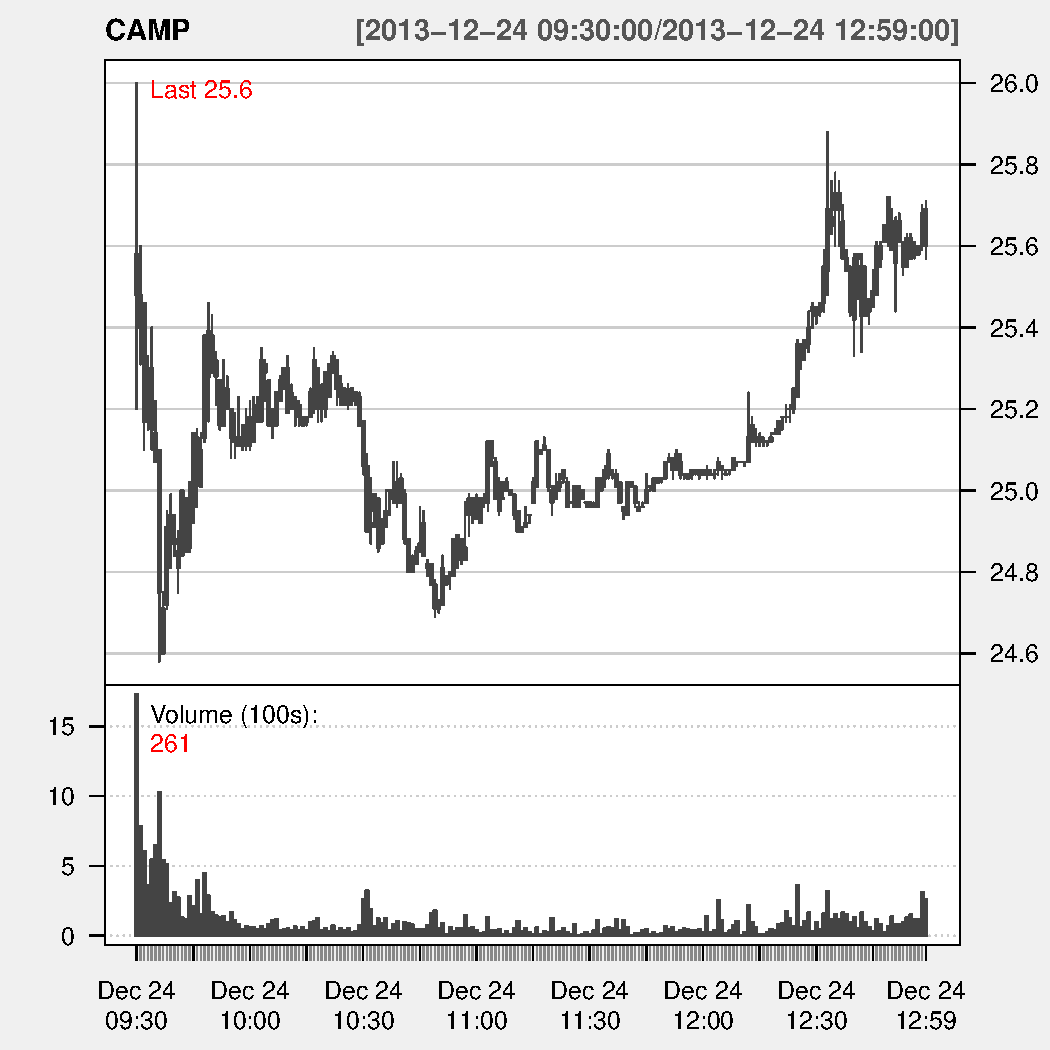
\includegraphics[width=\maxwidth]{/home/jhleong/dev/R/buy_on_gap/BuyOnGap_report/figure/price_chart} 

\end{knitrout}


\end{fullwidth}
\end{document}
